% !TeX root = ./poster.tex
% The MIT License (MIT)
% =====================

% **Copyright (c) 2018 Anish Athalye (me@anishathalye.com)**

% Permission is hereby granted, free of charge, to any person obtaining a copy of
% this software and associated documentation files (the "Software"), to deal in
% the Software without restriction, including without limitation the rights to
% use, copy, modify, merge, publish, distribute, sublicense, and/or sell copies
% of the Software, and to permit persons to whom the Software is furnished to do
% so, subject to the following conditions:

% The above copyright notice and this permission notice shall be included in all
% copies or substantial portions of the Software.

% THE SOFTWARE IS PROVIDED "AS IS", WITHOUT WARRANTY OF ANY KIND, EXPRESS OR
% IMPLIED, INCLUDING BUT NOT LIMITED TO THE WARRANTIES OF MERCHANTABILITY,
% FITNESS FOR A PARTICULAR PURPOSE AND NONINFRINGEMENT. IN NO EVENT SHALL THE
% AUTHORS OR COPYRIGHT HOLDERS BE LIABLE FOR ANY CLAIM, DAMAGES OR OTHER
% LIABILITY, WHETHER IN AN ACTION OF CONTRACT, TORT OR OTHERWISE, ARISING FROM,
% OUT OF OR IN CONNECTION WITH THE SOFTWARE OR THE USE OR OTHER DEALINGS IN THE
% SOFTWARE.


% Gemini theme
% https://github.com/anishathalye/gemini

\documentclass[final]{beamer}

% ====================
% Packages
% ====================

\usepackage[T1]{fontenc}
\usepackage{lmodern}
\usepackage[size=custom,width=130 ,height=100,scale=1.0]{beamerposter}
\usetheme{gemini}
\usecolortheme{gemini}
\usepackage{graphicx}
\usepackage{booktabs}
\usepackage{tikz}
\usepackage{pgfplots}
\usepackage{tcolorbox}
\usepackage{geometry}

% ====================
% Lengths
% ====================

% If you have N columns, choose \sepwidth and \colwidth such that
% (N+1)*\sepwidth + N*\colwidth = \paperwidth
\newlength{\sepwidth}
\newlength{\colwidth}
\setlength{\sepwidth}{0.025\paperwidth}
\setlength{\colwidth}{0.3\paperwidth}

\newcommand{\separatorcolumn}{\begin{column}{\sepwidth}\end{column}}

% ====================
% Title
% ====================

\title{Ileum microbiota composition and inflammatory response\\ in triple transgenic mice modeling Alzheimer's disease}

\author{Kathryn Conn \textsuperscript{*} \and Christopher R. Keefe \textsuperscript{*} \and Emily Borsom \and Allyson Hirsh \and Melanie Palma Avila \and J. Gregory Caporaso \textsuperscript{†} \and Emily K. Cope \textsuperscript{†} }

\institute[shortinst]{The Pathogen and Microbiome Institute at Northern Arizona University \\
{\footnotesize \textsuperscript{*} Equal Contributors \hskip .5cm \textsuperscript{†} Advisors} }

% ====================
% Body
% ====================

\begin{document}

\begin{frame}[t]
\begin{columns}[t]
\separatorcolumn

\begin{column}{\colwidth}

% TODO: remove
% \begin{block}{Abstract}
%   Alzheimer’s disease (AD), a neurodegenerative disease that affects 1 in 10
%   adults over 65 in the United States, is characterized by neuroinflammation,
%   neurofibrillary tangles, and aggregated amyloid-β plaques in the brain.
%   These key pathologies lead to debilitating symptoms including impaired
%   cognitive function and memory loss. Recent studies indicate a correlation
%   between the gut microbiota and AD, which may be due to mechanisms such as
%   increased inflammatory responses that aggravate neuroinflammation. The gut
%   microbiota is the aggregate of all microbial life resident in the
%   gastrointestinal tract. This bidirectional communication between gut
%   microbes and the brain is known as the gut microbiota-brain axis. By
%   identifying the microbial communities resident in the ileum of triple
%   transgenic mice modeling AD pathologies (3xTg-AD), we can understand
%   correlations between key microbial taxa and AD pathogenesis. In this
%   research, we evaluated the ileum microbiota and inflammatory responses of
%   triple transgenic AD mice compared to wild-type control mice. The ileum is
%   the most distal region of the small intestine and a known site for immune
%   modulation due to the presence of lymph nodules known as Peyer’s patches.
%   Analysis of ileum microbiota composition was performed by sequencing the V4
%   region of the 16S rRNA gene. Microbiome bioinformatics was performed using
%   QIIME 2. Inflammatory responses were quantified using reverse transcriptase
%   quantitative polymerase chain reaction (RT-qPCR) with targeted gene primers
%   and statistical analysis was performed using Prism. We expect to see mice
%   genetically predisposed to developing AD pathologies exhibit a decreased
%   species richness and altered composition of the ileum microbiome and
%   upregulation of proinflammatory cytokines. These studies will provide a
%   critical link between the ileum microbiome, inflammation, and AD, and will
%   contribute to development of microbiota-based therapeutics for AD.
% \end{block}

\begin{block}{Objective and Introduction}

    \textbf{Objective:} To correlate features of the microbial communities
    resident in the ileum of triple transgenic mice modeling AD pathologies
    (3xTg-AD) with Alzheimer's Disease (AD) pathogenesis.

    \textbf{Relevant Context:}
    \begin{itemize}
      \item AD is a neurodegenerative disease that affects 1 in 10 adults over 65 in the United States
      \item The gut microbiota is the aggregate of all microbial life resident in the gastrointestinal tract.
      \item The ileum, the most distal region of the small intestine, is a known site for immune modulation
      \item Studies correlate gut microbiome characteristics and AD pathology, possibly facilitated by bidirectional communication between gut microbes and the brain along the 'gut-brain axis'
      \item AD is characterized by neuroinflammation, neurofibrillary tangles, and aggregated amyloid-β plaques in the brain.
      \item These pathologies may be influenced by inflammatory cytokines produced in the gut.
    \end{itemize}

    \textbf{Hypothesis:}
    We expect to see mice genetically predisposed to developing AD
    pathologies exhibit altered composition of the ileum microbiome and
    upregulation of proinflammatory cytokines.
      
  \end{block}

  \begin{block}{Laboratory Methods}

  \begin{figure}[tph!]
    {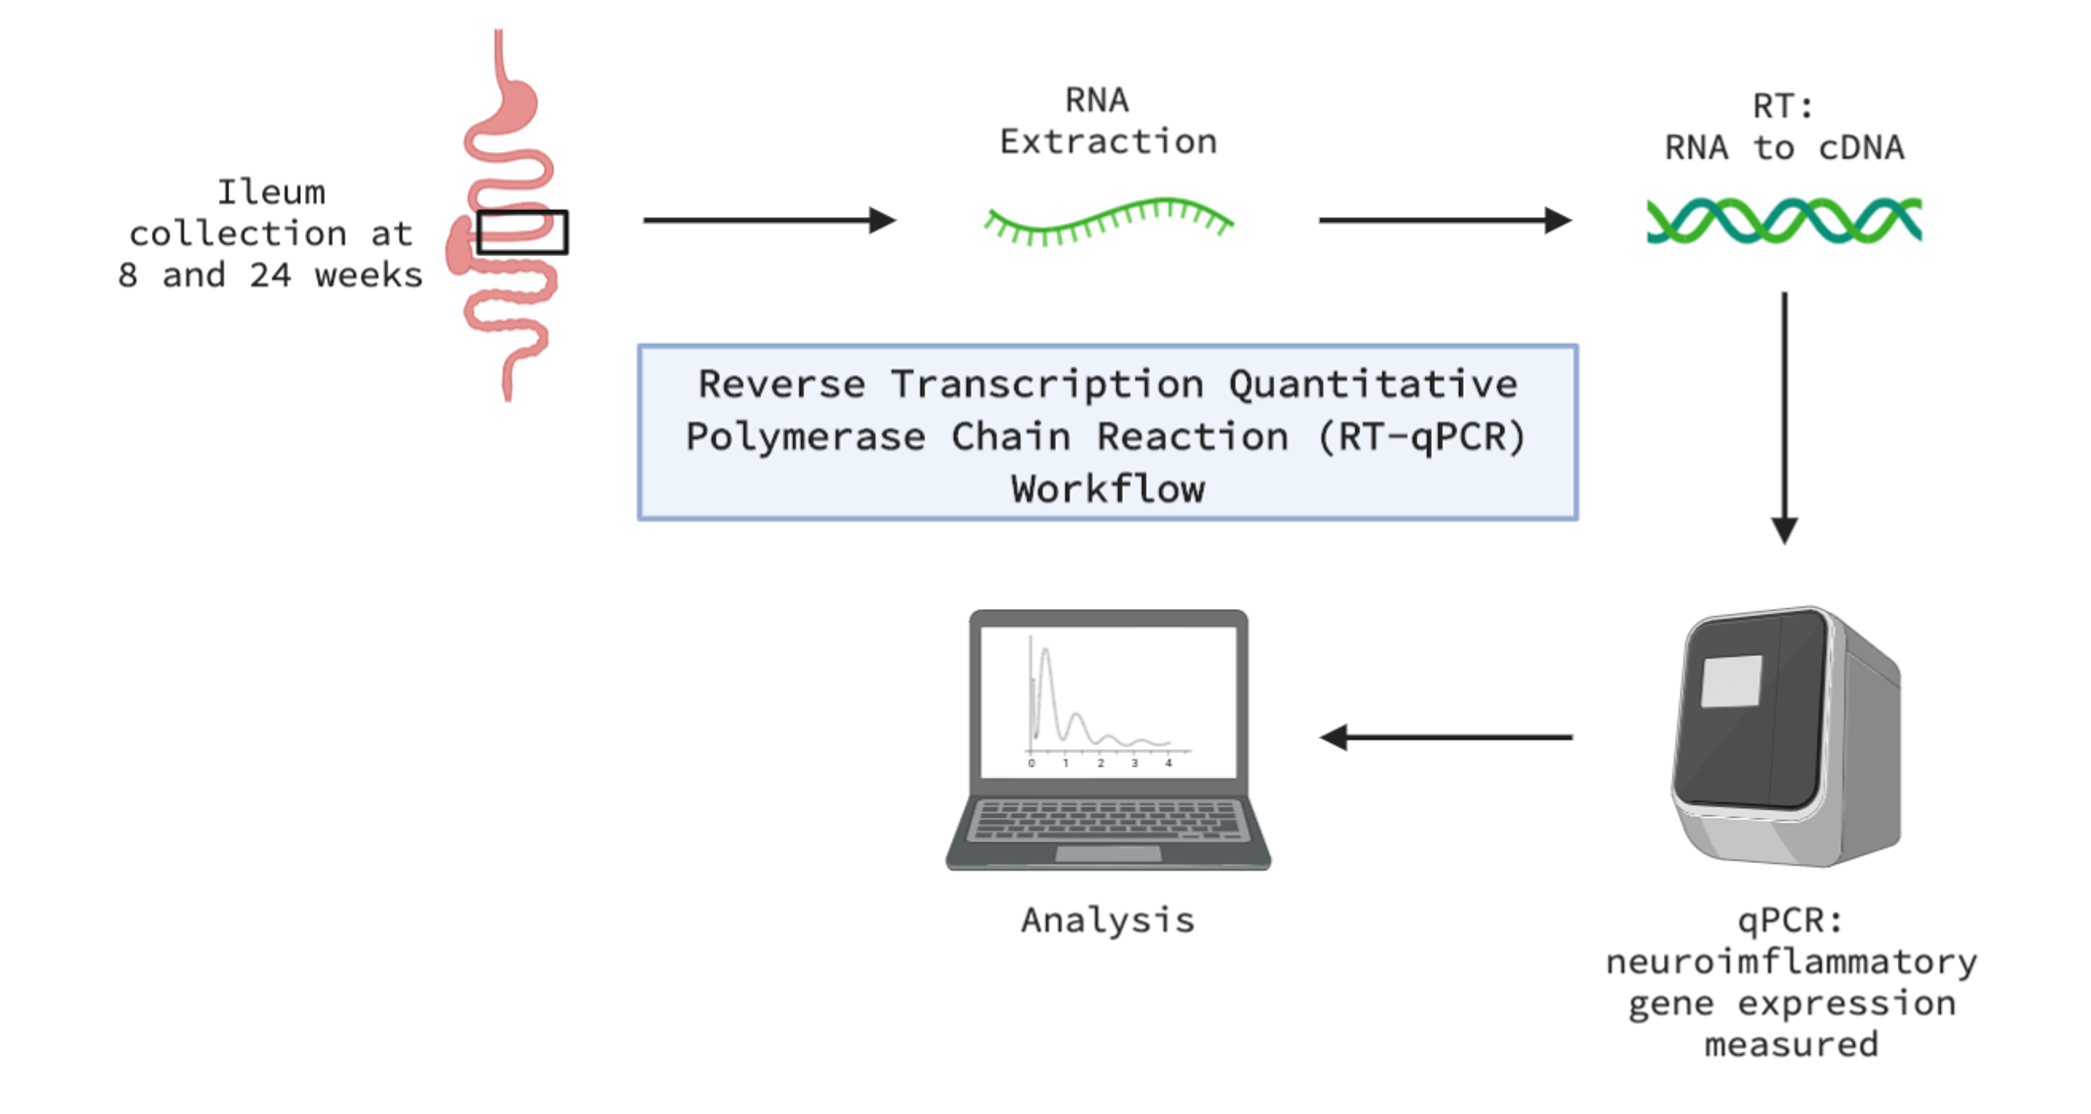
\includegraphics[height=14cm]{assets/qPCR_methods}}
    \caption{Visual rendering of qPCR wet lab processes. Samples are collected at 8, 24, and 52 weeks. RNA is extracted and reverse transcribed to cDNA. cDNA undergoes qPCR, and the resulting data is analyzed.}
    \label{fig:qpcrMethods}
  \end{figure}

  \begin{figure}[tph!]
    {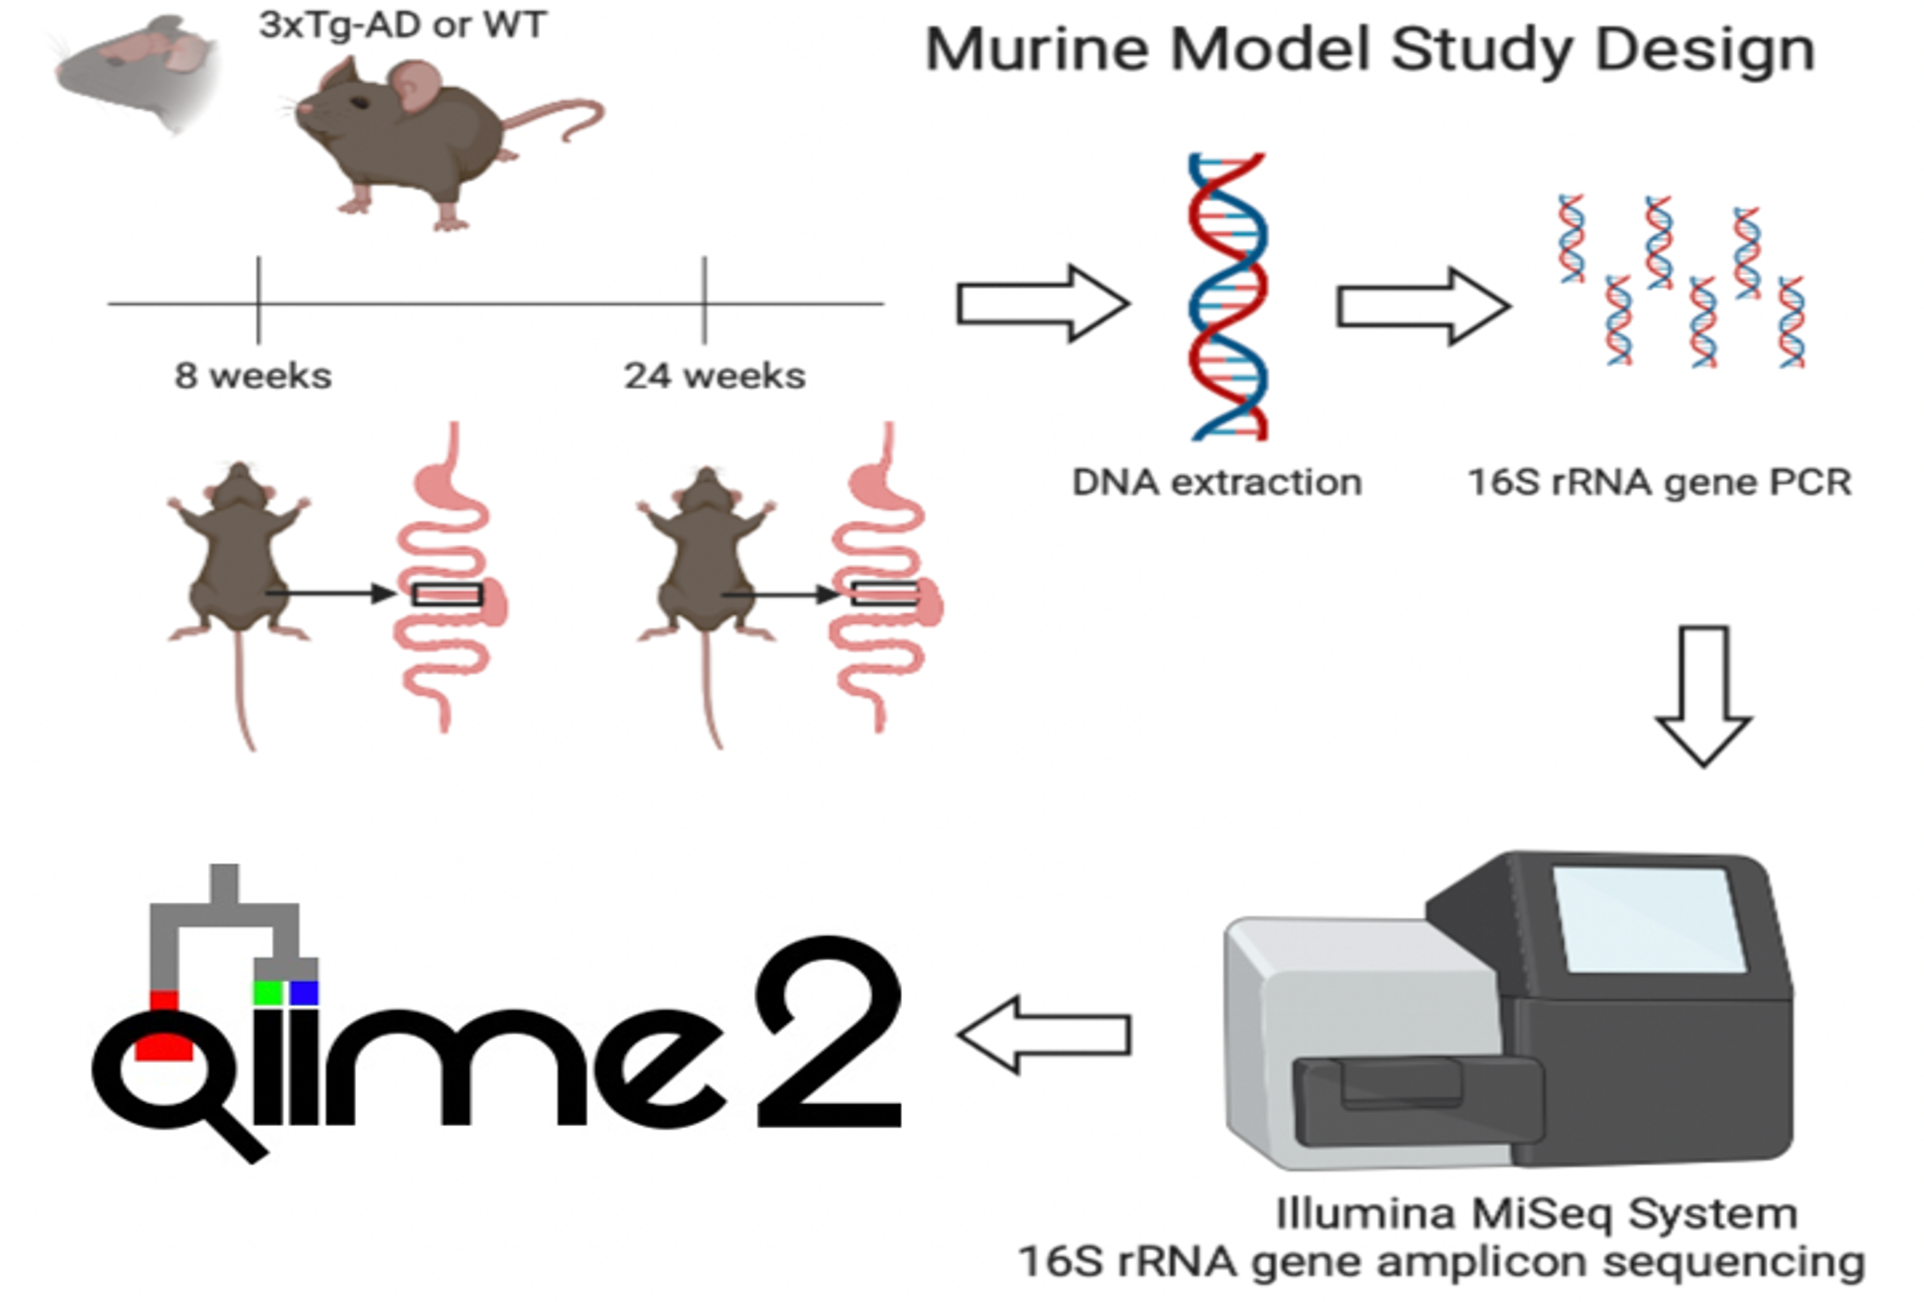
\includegraphics[height=14cm]{assets/16s_lab_methods}}
    \caption{Visual rendering of 16s wet lab processes. Samples are collected at 8, 24, and 52 weeks. DNA is extracted and 16s rRNA is transcribed from it. Sequencing is performed with an Illumina MiSeq, and the resulting data is analyzed with QIIME 2.}
    \label{fig:16sMethods}
  \end{figure}

  \end{block}

  \begin{block}{Bioinformatics Methods}

    Analysis of 16s rRNA data was performed with QIIME 2 2020.2 (Bolyen et al. 2019).
    \begin{itemize}
      \item {sequence data demultiplexing and quality filtering: \code{q2‐demux}}
      \item {denoising to amplicon sequence variants (ASVs): DADA2 (Callahan et al. 2016) (via \code{q2‐dada2})}
      \item {phylogeny constructed by inserting ASVs into a greengenes 13\_8 reference database using SEPP (via \code{q2‐fragment-insertion})}
      \item {taxonomic annotations assigned from greengenes 13\_8 99\% OTUs (McDonald et al. 2012) using \code{q2‐feature‐classifier classify-sklearn} (Bokulich et al. 2018a).}
      \item {unequal sampling depths were normalized by rarefying to 13102 sequences per sample}
      \item {diversity analysis \code{q2-diversity} \code{q2-emperor} and \code{q2-longitudinal}}
      \item {differential abundance: ANCOM via \code{q2-composition}}
    \end{itemize}

    Analysis of qPCR data was performed with Microsoft Excel and GraphPad Prism
    \begin{itemize}
      \item {Raw data normalized to Relative Quantification (RQ) AKA "fold change"}
      \item {RQ data is grouped by Strain and sample collection time point}
      \item {RQ per sample is plotted for each amplified cytokine}
    \end{itemize} 

  \end{block}

\end{column}

\separatorcolumn

\begin{column}{\colwidth}

  \begin{block}{Visualizations}

    % Use this figure if we want Arg1 and Nos2 figures side-by-side
    \begin{figure}[!htb]
      \minipage{0.48\textwidth}%
        \begin{center}
          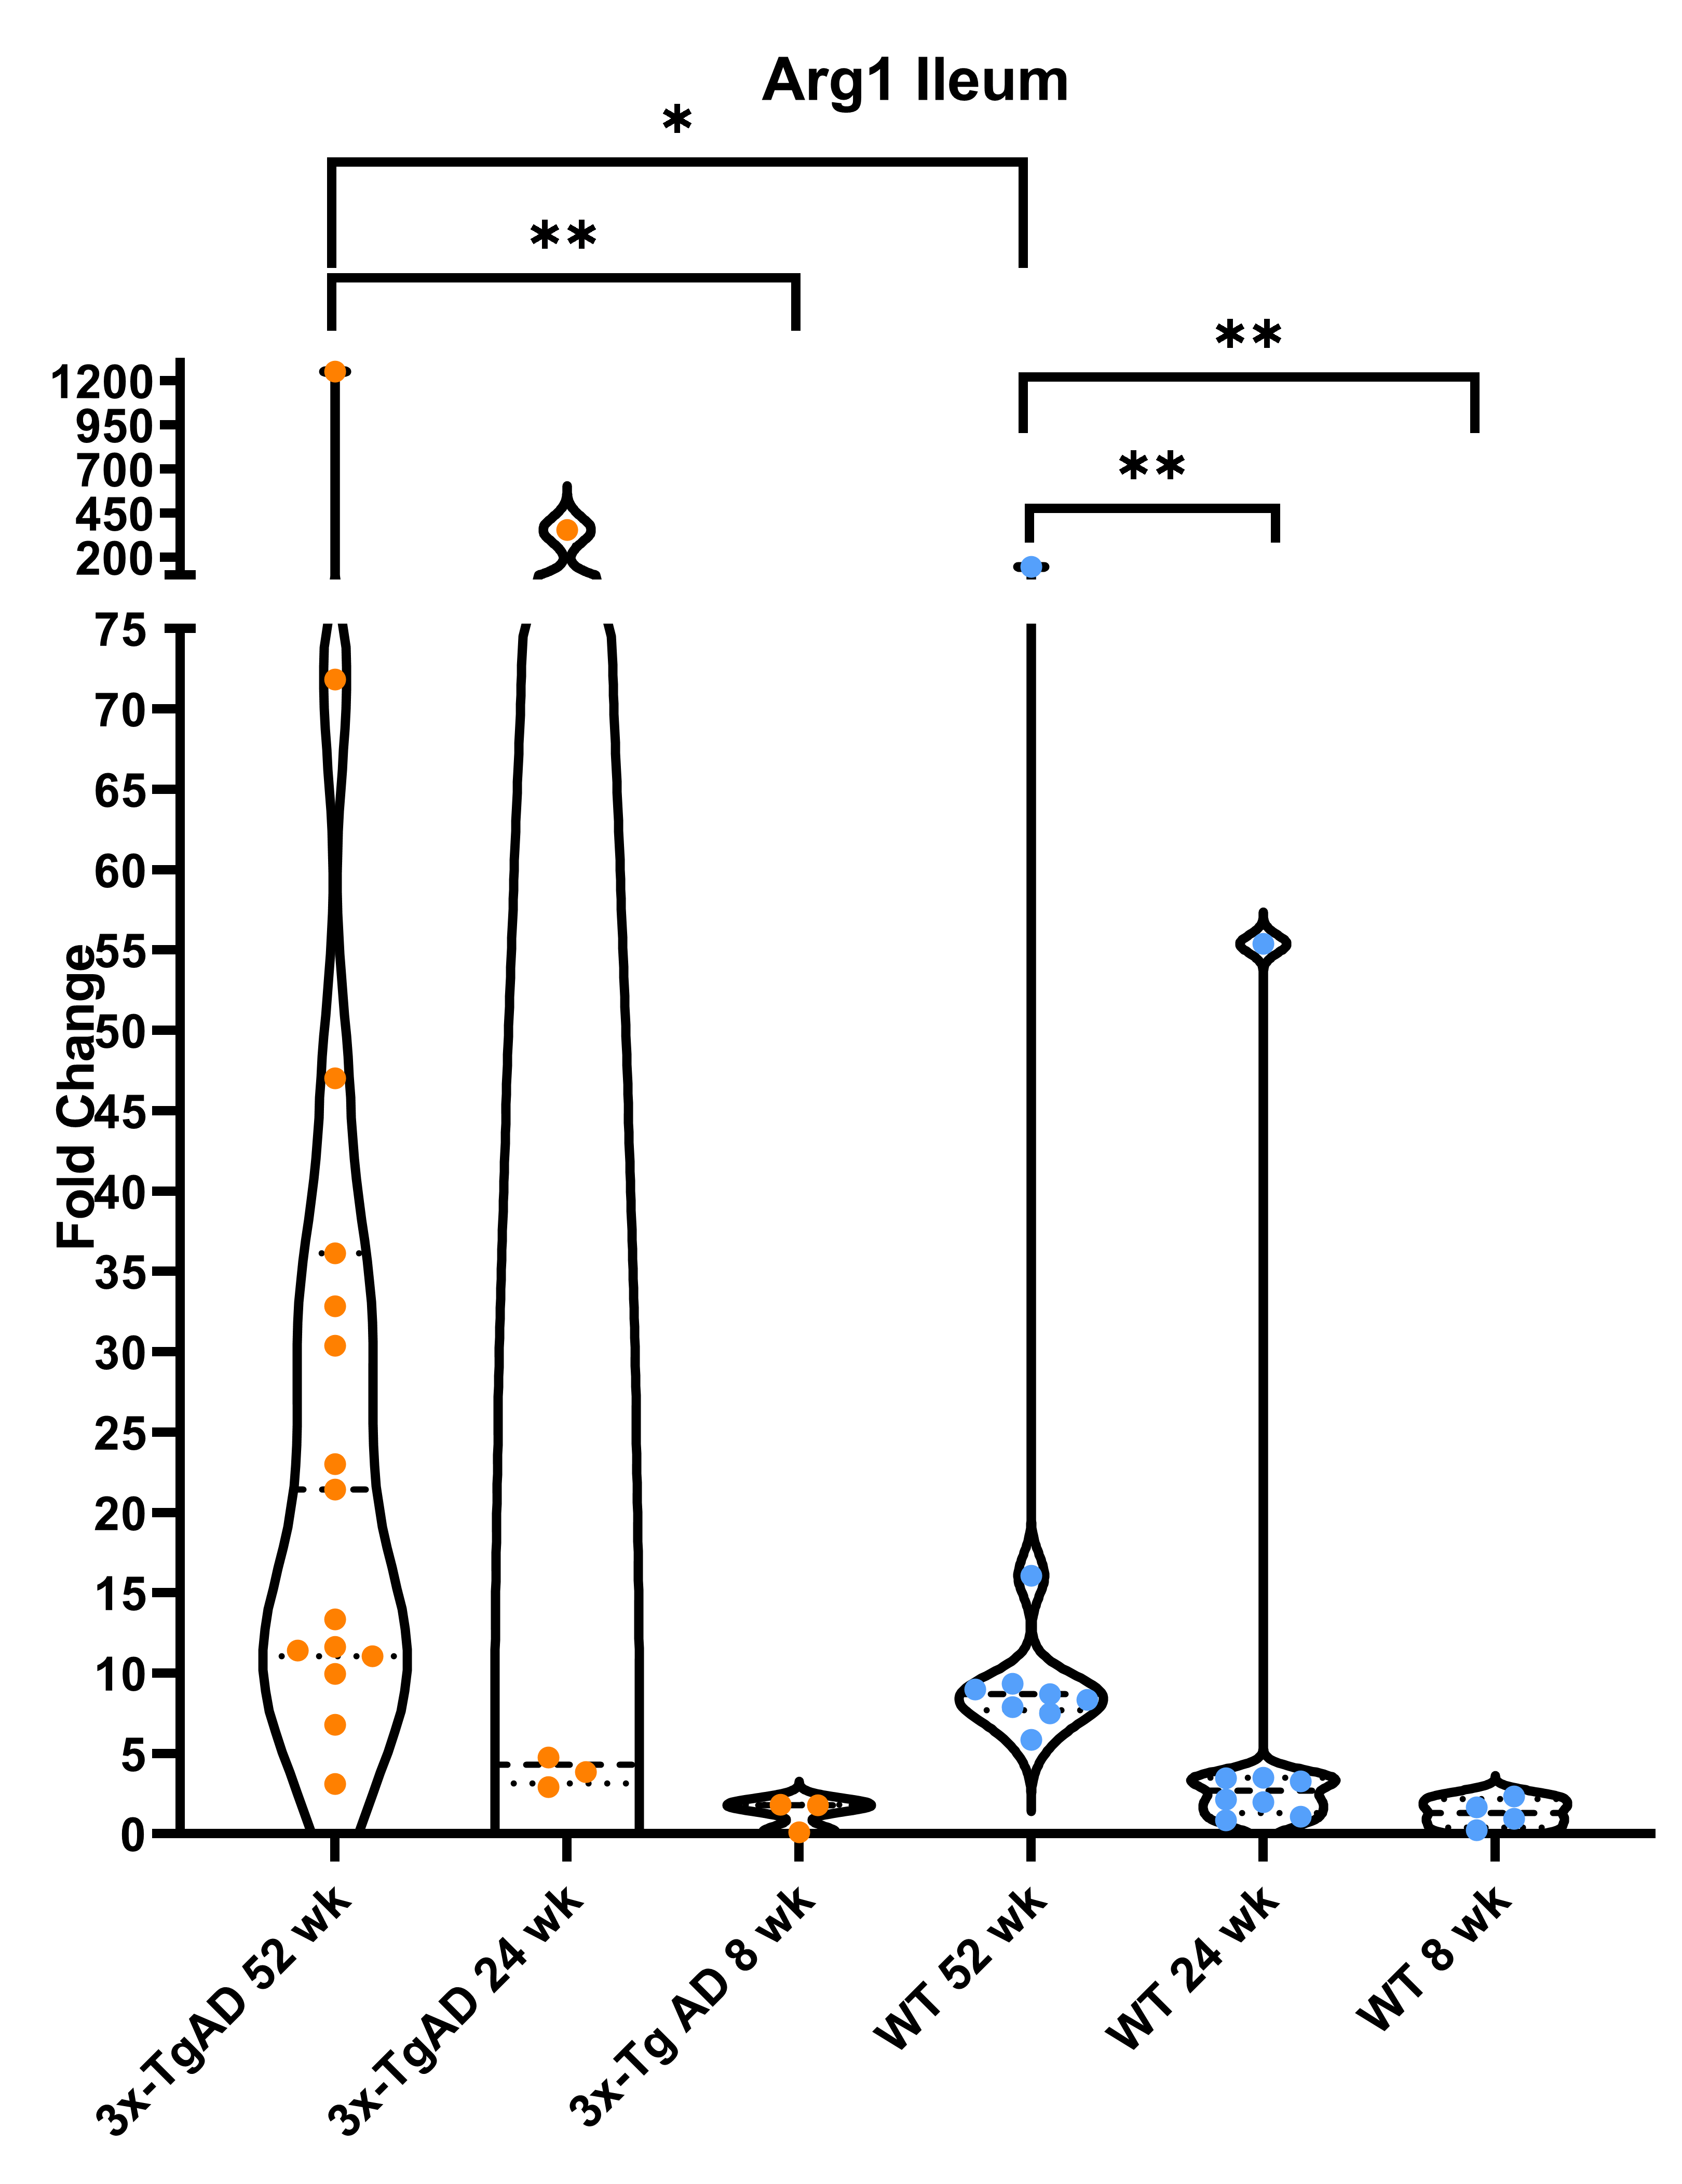
\includegraphics[width=\linewidth]{assets/arg1_Ileum}
        \end{center}
      \endminipage
      % \hskip 1cm
      \minipage{0.48\textwidth}
        \begin{center}
          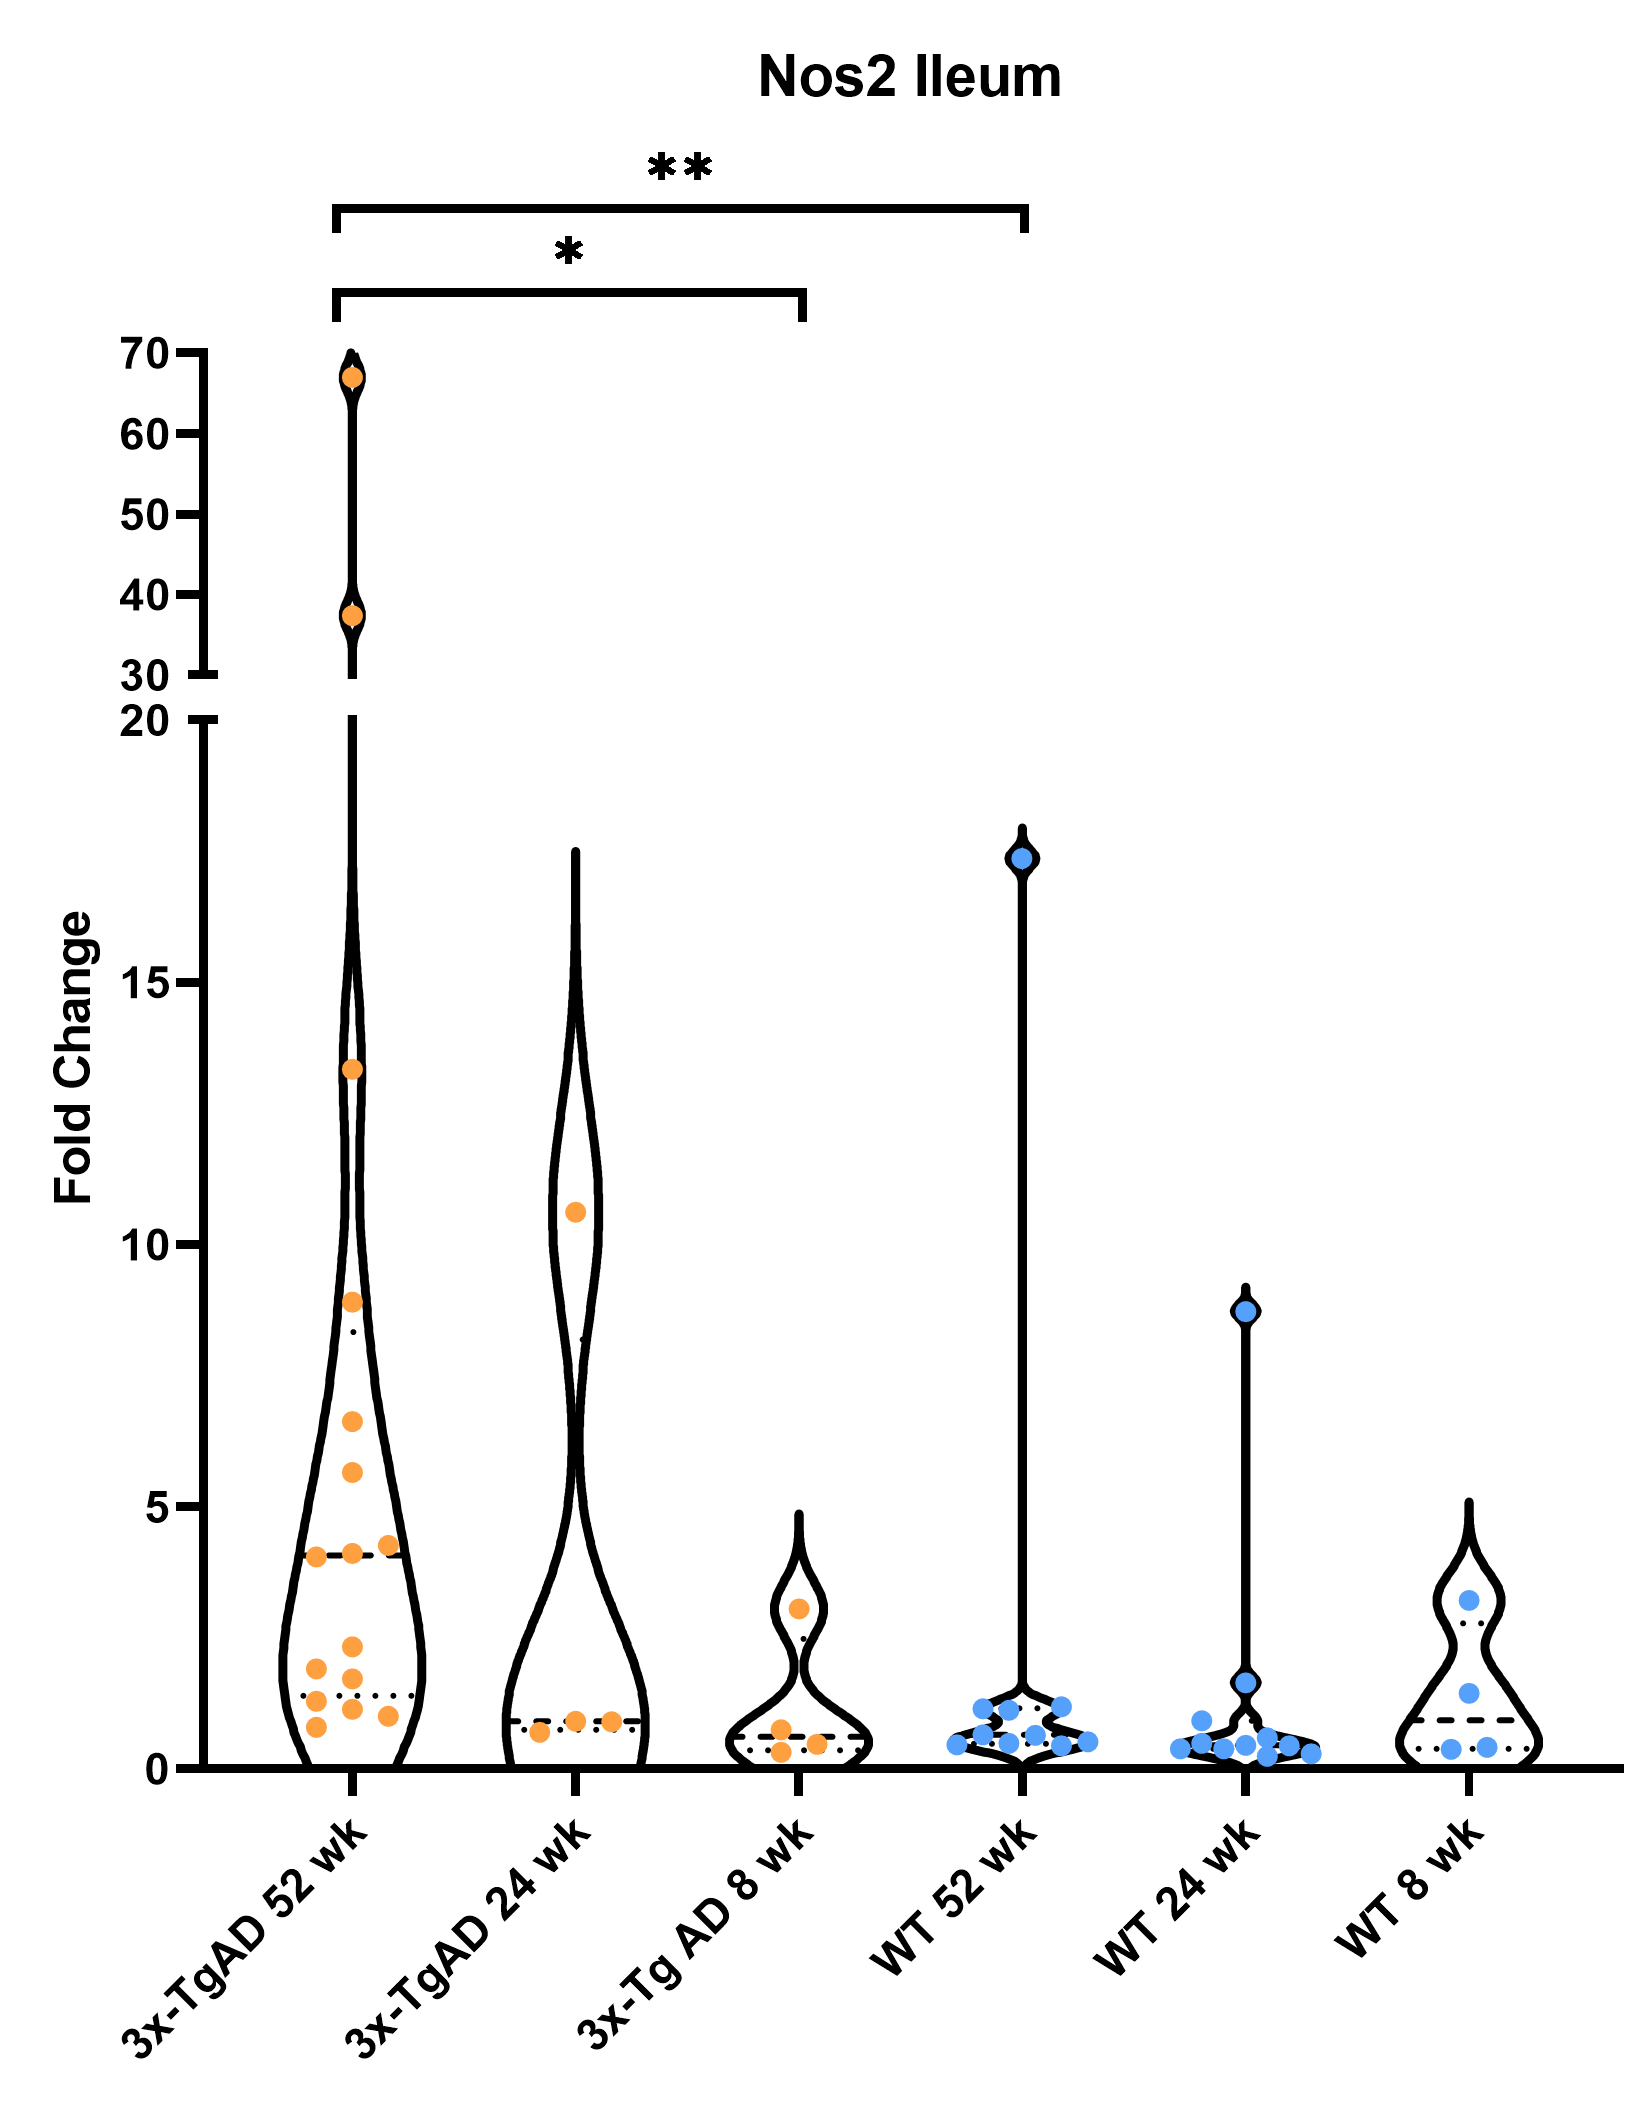
\includegraphics[width=\linewidth]{assets/nos2_Ileum}
        \end{center}
      \endminipage\hfill
      \caption{\,Gene expression of cytokines Arg1 and Nos2 is significantly increased in 3xTg-AD mice over WT mice. Significant differences exist in gene expression of cytokines Arg1 and Nos2 between 8 weeks and 52 weeks of age (Mann-Witney p<0.05).}
      \label{fig:qpcrResults}
    \end{figure}

    % Use these figures if we want to stack Arg1 and Nos2 figures vertically
    % \begin{figure}[tph!]
    %   {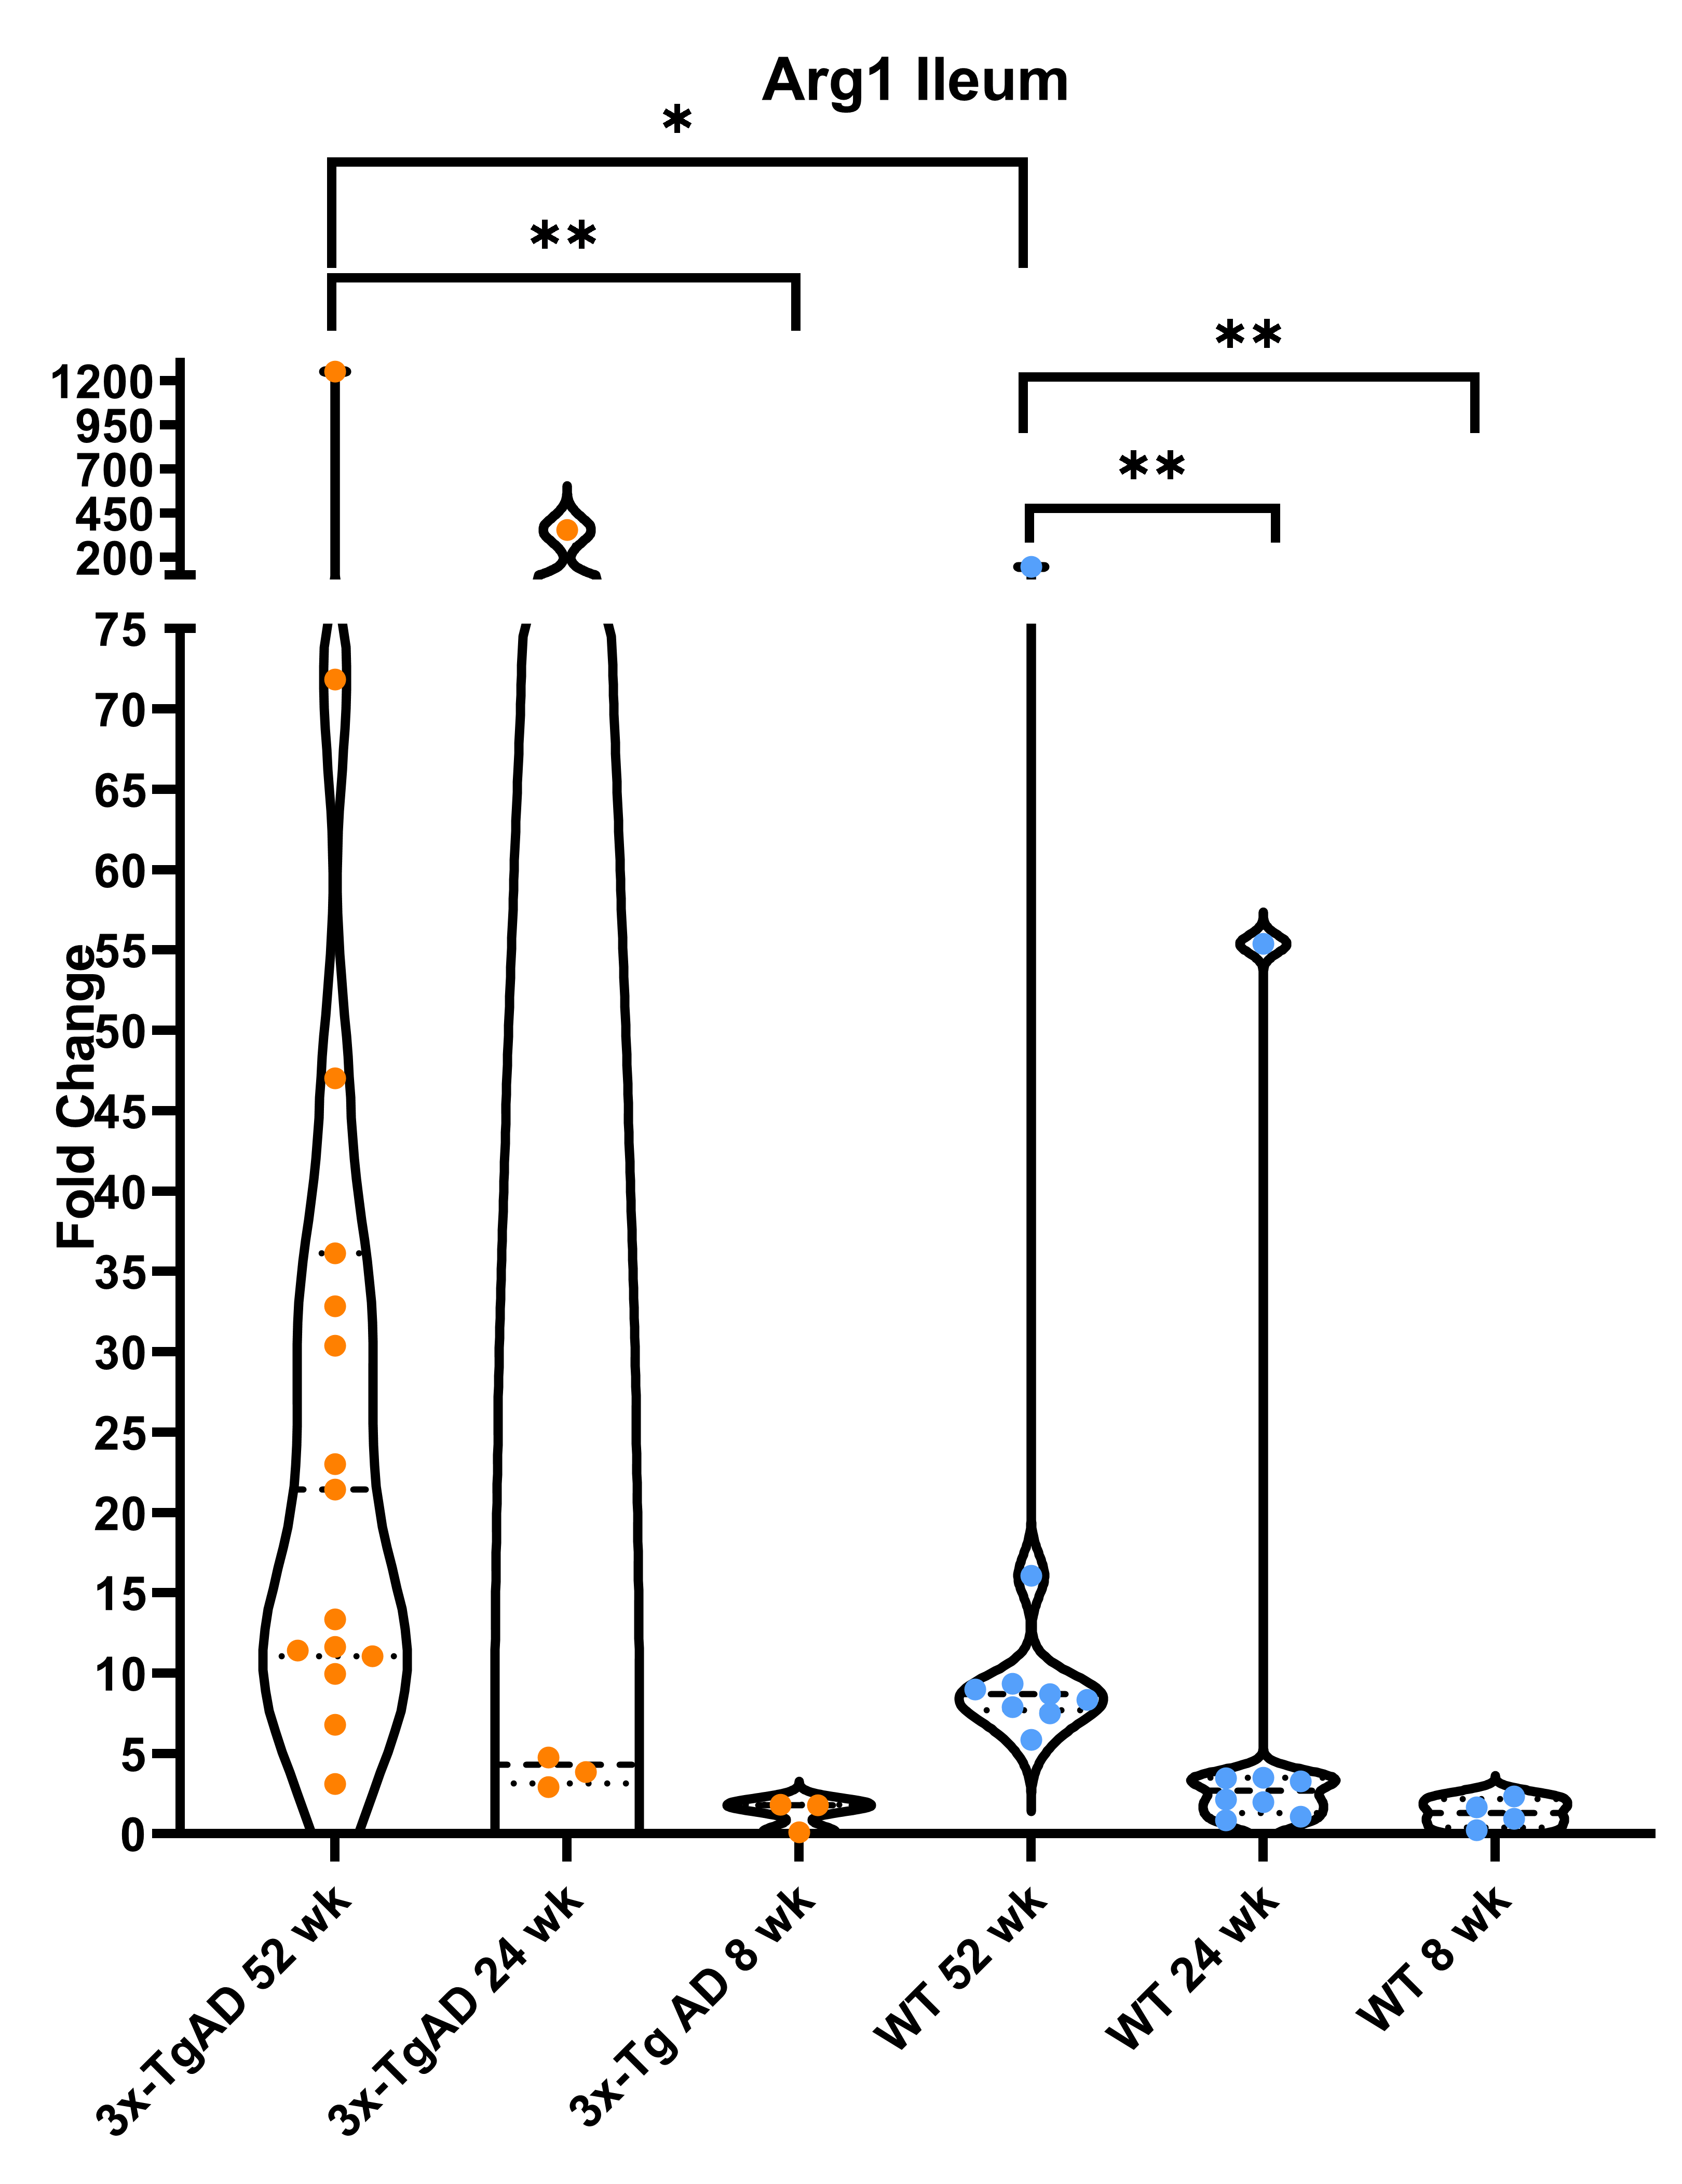
\includegraphics[height=20cm]{assets/arg1_Ileum}}
    %   \caption{\,Provenance tree describing the production of our taxonomic bar plot visualization. QR code provides interactive access to both provenance tree and bar plot (Figure 4).}
    %   \label{fig:provenance}
    % \end{figure}

    % \begin{figure}[tph!]
    %   {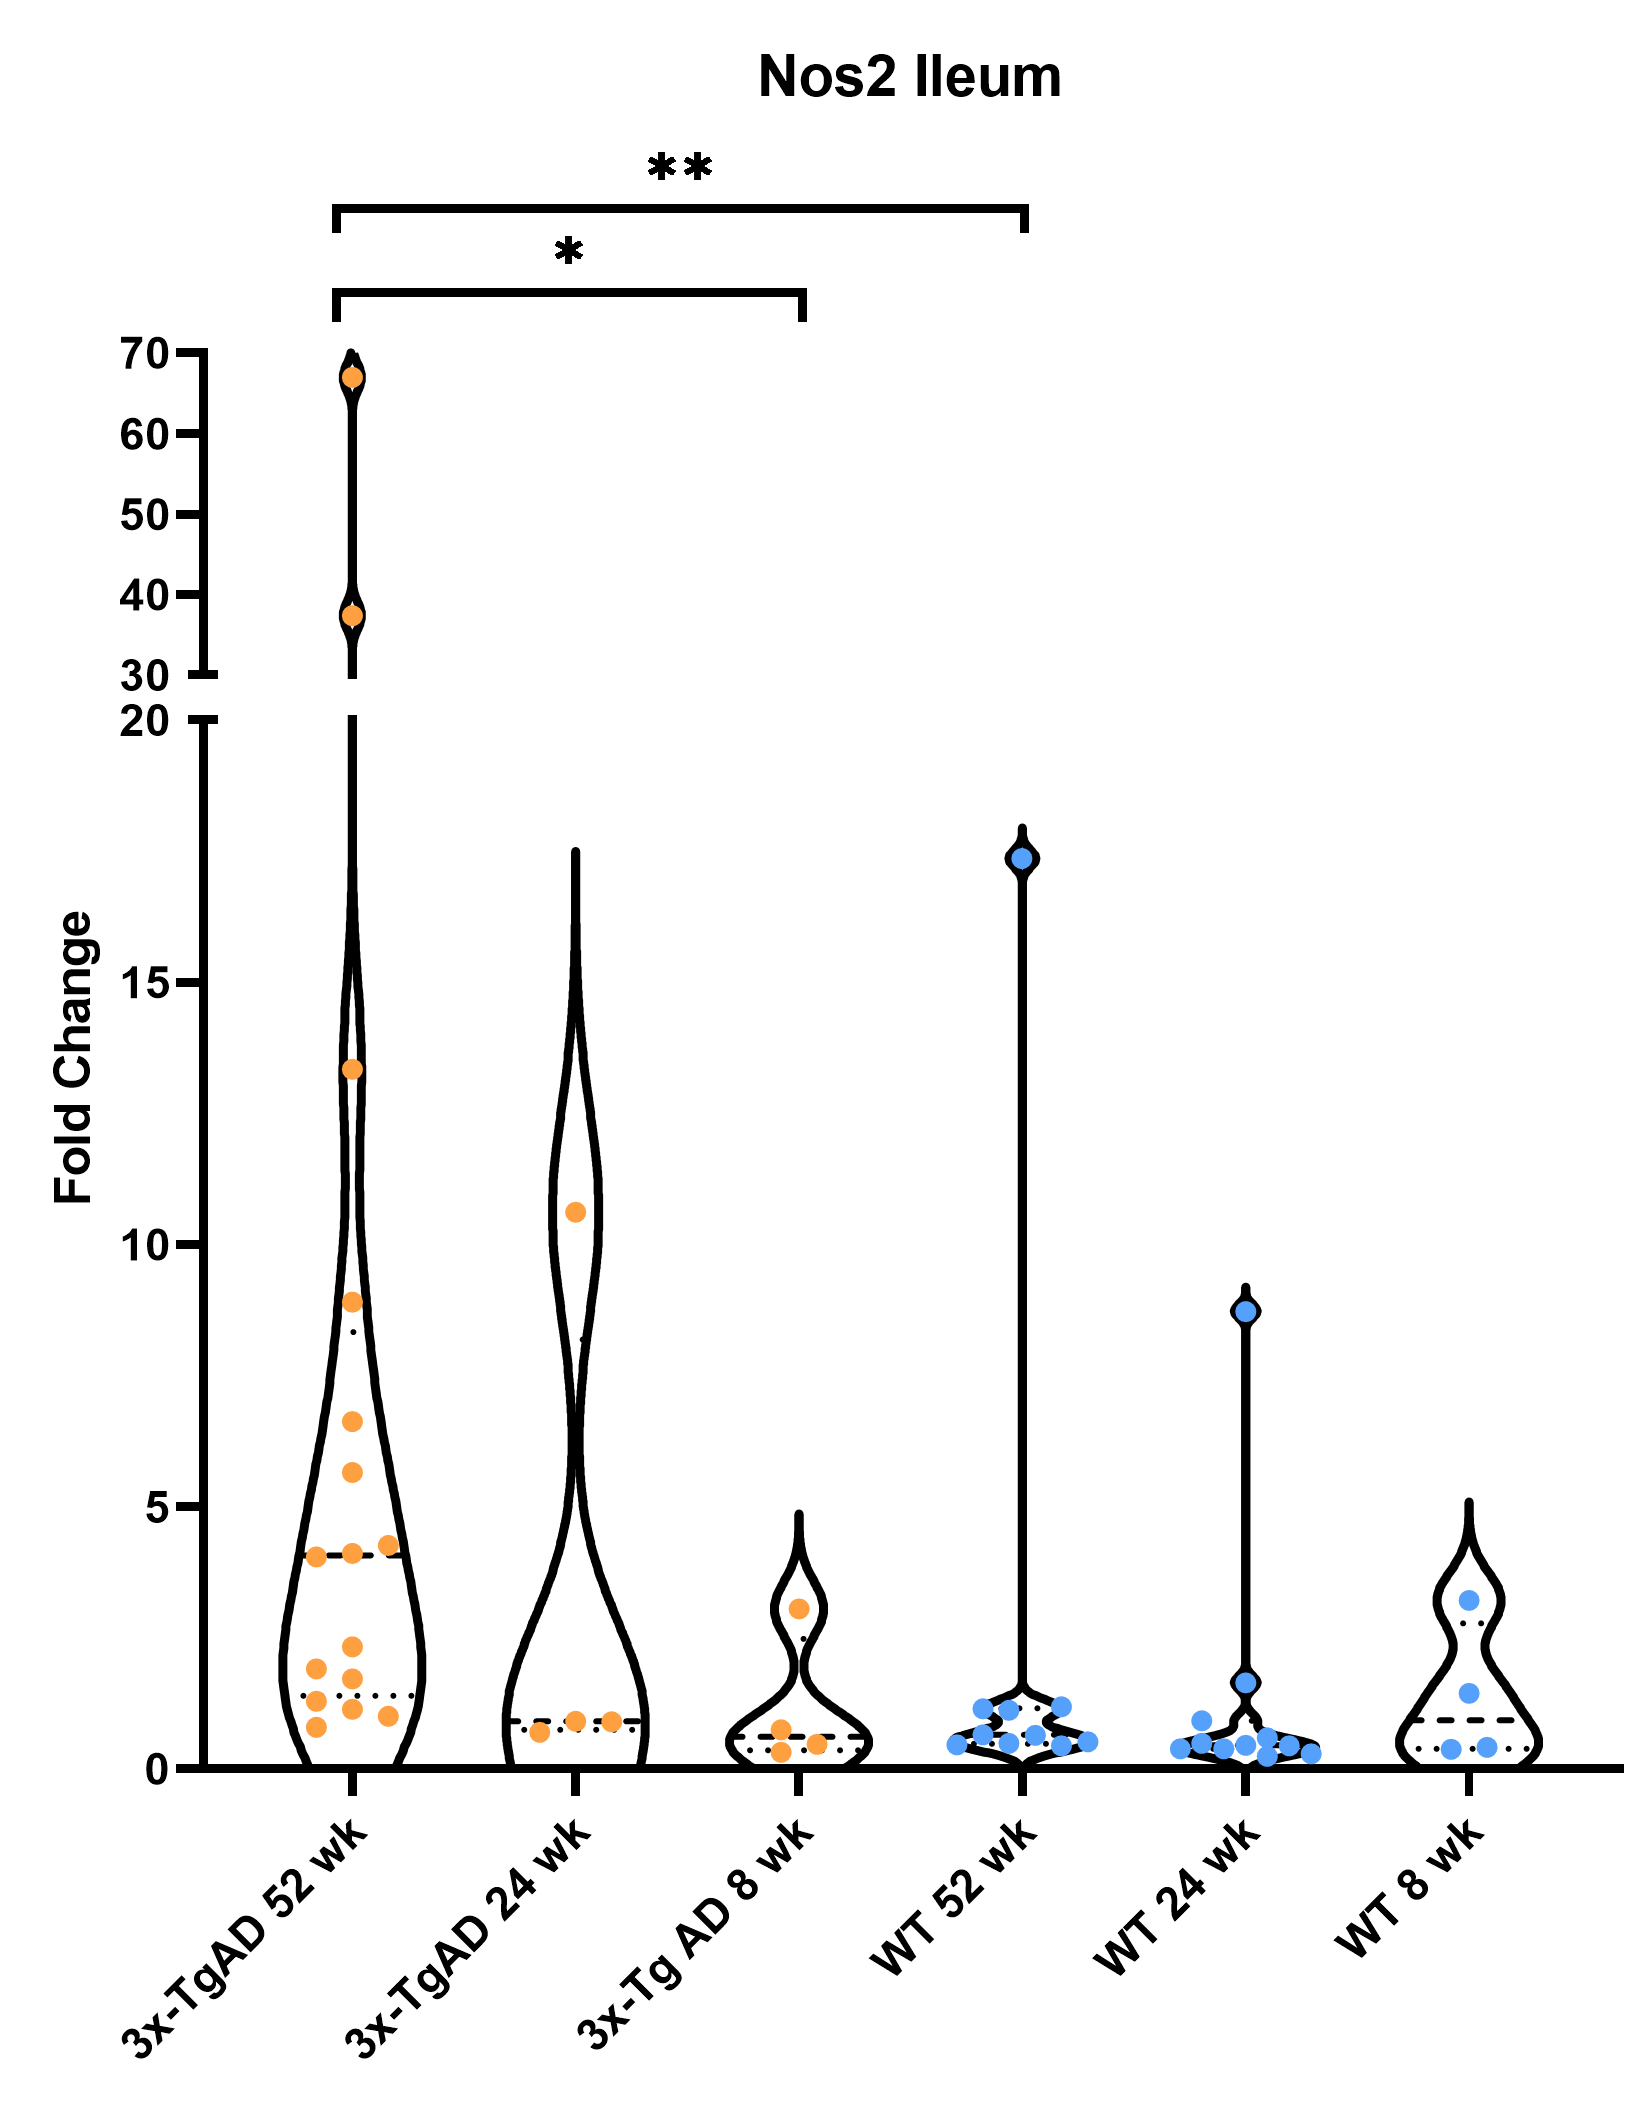
\includegraphics[height=20cm]{assets/nos2_Ileum}}
    %   \caption{\,Taxonomic bar plot sorted by Average Soil Relative Humidity on the x-axis }
    %   \label{fig:taxabar-plot}
    % \end{figure}

    \begin{figure}[tph!]
      {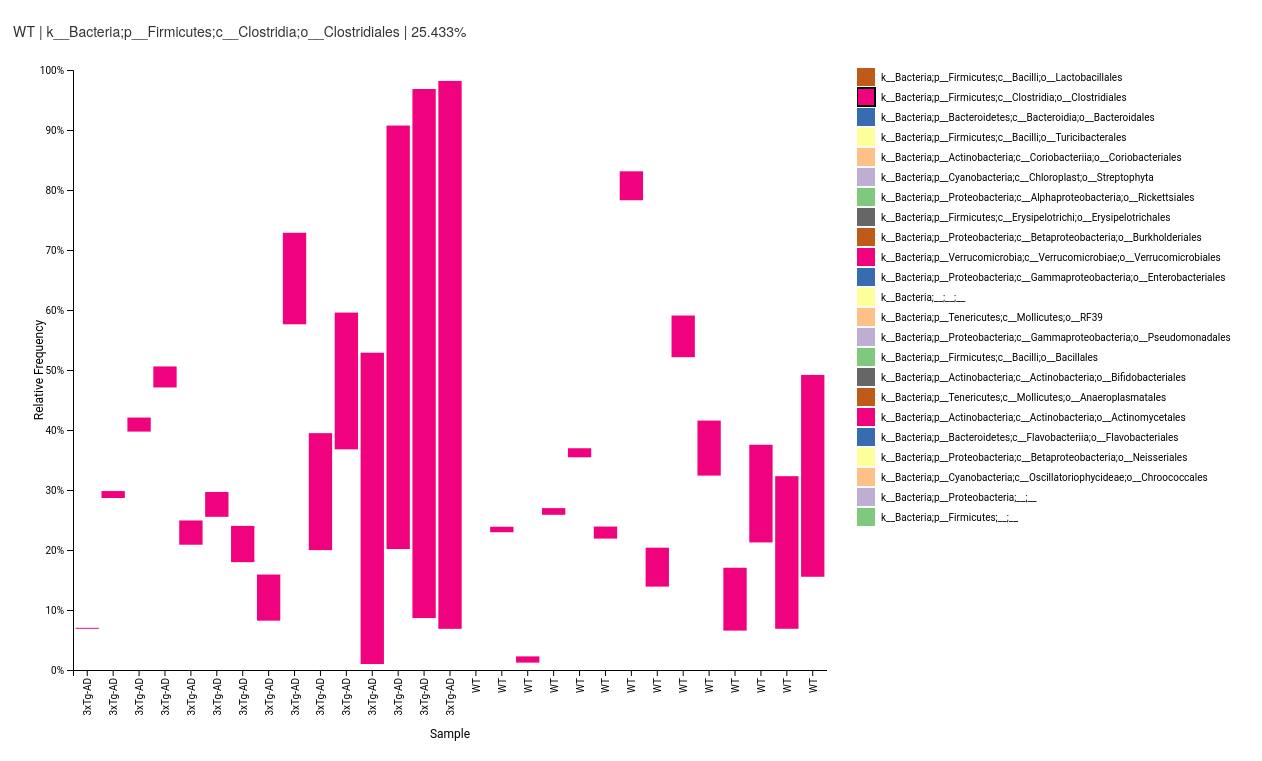
\includegraphics[height=20cm]{assets/taxa_barplot}}
      \caption{\,A plot of taxa present per sample, collapsed at the Order
      level, seems to indicate higher prevalence of Clostridiales in
      transgenic "Alzheimer’s" mice, but differential abundance testing with
      ANCOM finds no significant differences across strains.}
      \label{fig:q2studio}
    \end{figure}
  \end{block}

  \begin{figure}[!htb]
      \minipage{0.48\textwidth}%
        \begin{center}
          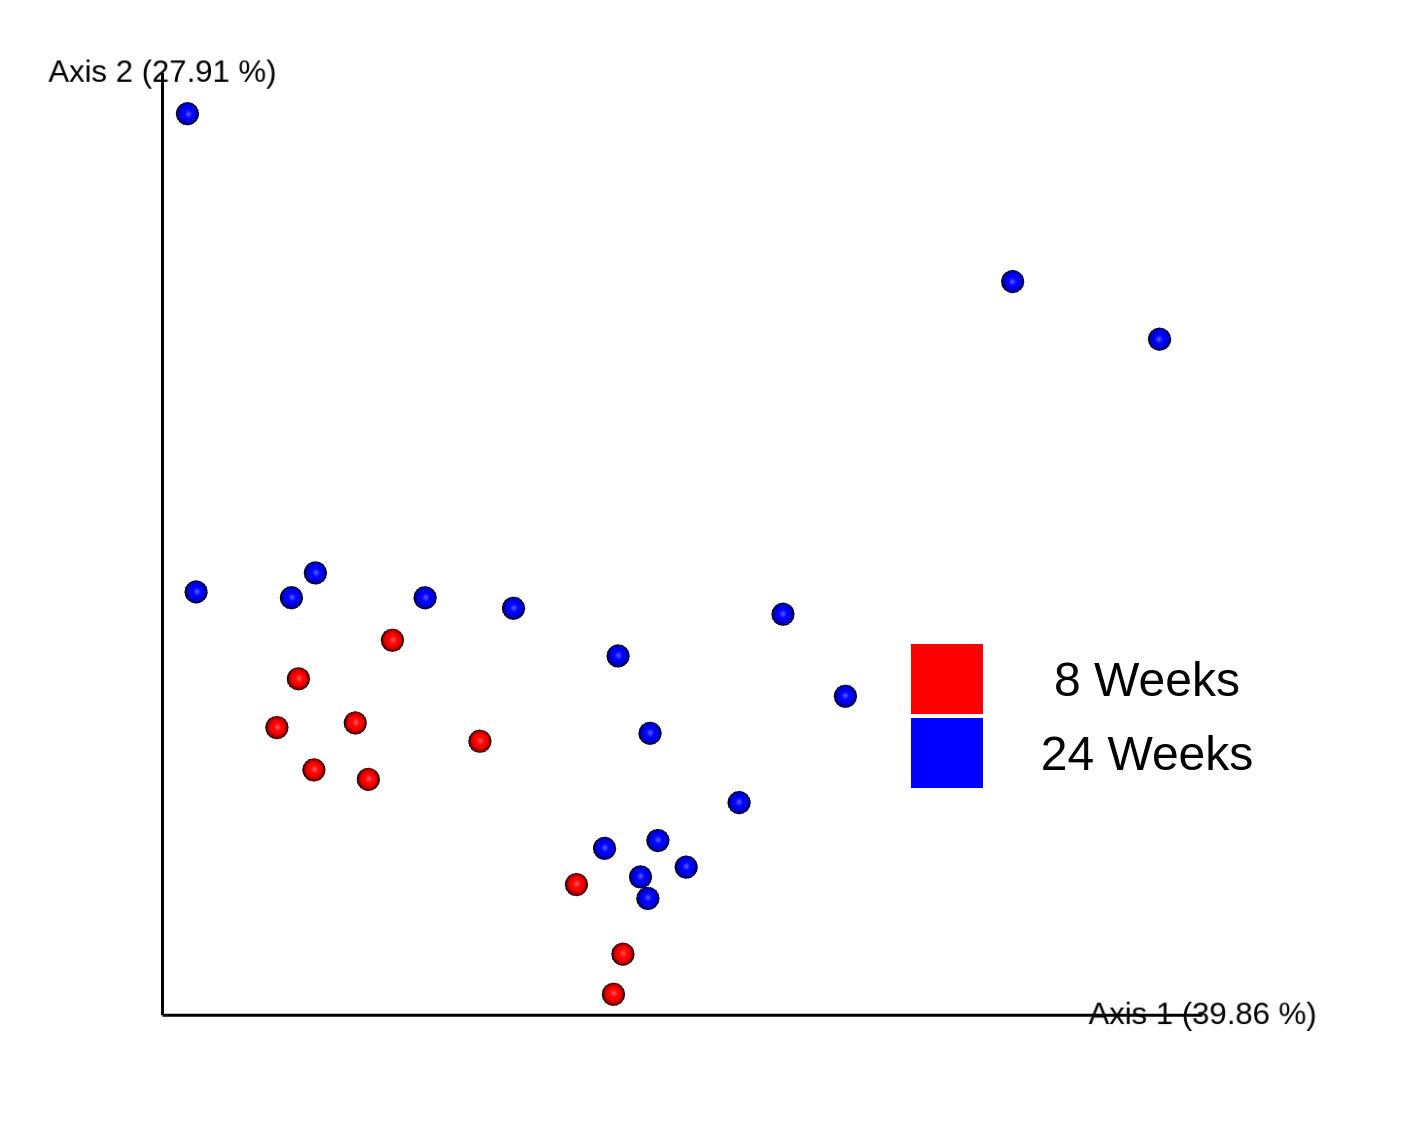
\includegraphics[width=\linewidth]{assets/w_unifrac_age_wk}
        \end{center}
      \endminipage
      \minipage{0.48\textwidth}
        \begin{center}
          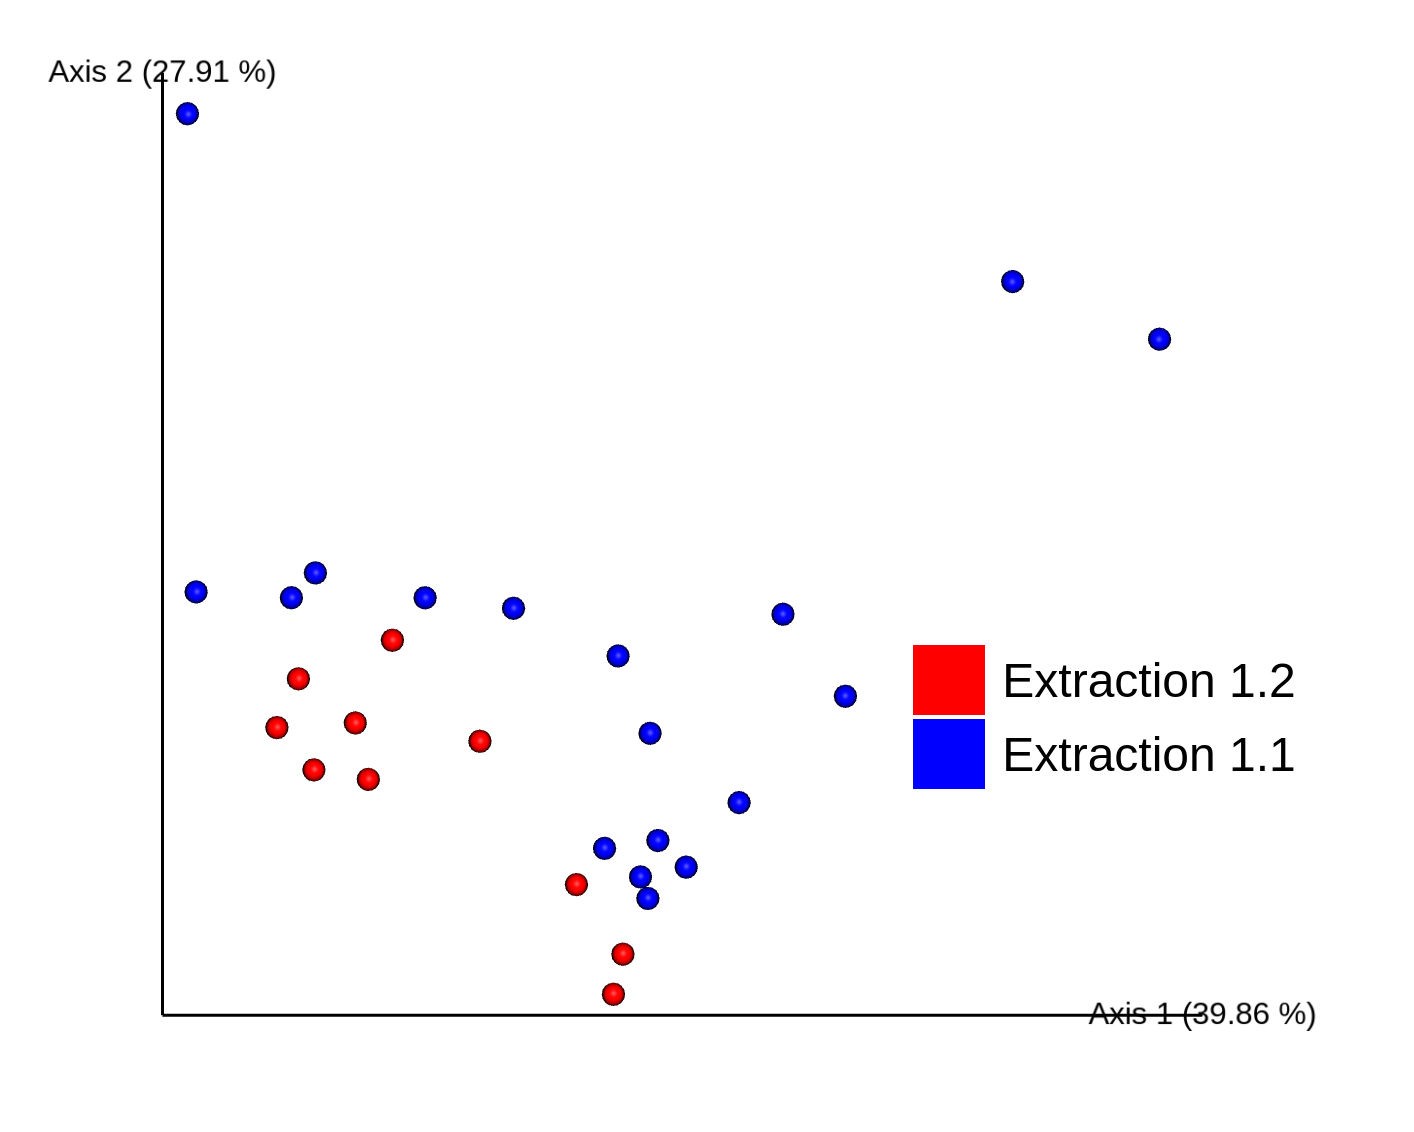
\includegraphics[width=\linewidth]{assets/w_unifrac_extraction}
        \end{center}
      \endminipage\hfill
      \caption{Weighted Unifrac PCoA plots colored on "age in weeks" and
      "extraction" show meaningful separation. They also show that all 8-week
      samples were extracted together, as were all 24-weeks samples,
      complicating interpretation.}
      \label{fig:qpcrResults}
    \end{figure}

  \begin{block}{Project Funding}
    This work was supported in part by the 2020-21 Urdea Collaborative
    Research Award Program to Kathryn Conn and Chris Keefe, through the
    Northern Arizona University Office of Undergraduate Research \& Creative
    Activity, and by the Arizona Alzheimer’s Consortium (Award number
    CTR040636) to Emily Cope and Greg Caporaso.
  \end{block}

\end{column}

\separatorcolumn

\begin{column}{\colwidth}
    \begin{block}{Results}
      \textbf{qPCR results:}
      \begin{itemize}
        \item Humanized 3xTg-AD mice express significantly higher levels of Arg1 and Nos2 cytokines than paired Wild Type mice
        \item Arg1 and Nos2 cytokines are expressed at significantly higher levels at 52 weeks than at 8 weeks
      \end{itemize}

      \textbf{16s results:}
      \begin{itemize}
      \item at 8 and 24 weeks, we see no statistically significant differences in alpha or beta diversity on Strain
      \item We see significant difference on age-week, but our extraction scheme may confound these results*
      \item Order Erysipelotrichales is the most important taxon in describing change over time from 8->24 weeks
      \end{itemize}

    \begin{tcolorbox}
    [width=\textwidth, colframe=blue]
      * DNA was extracted from all 8-week samples in one batch, and all
      24-weeks samples in another. Though we find significant changes in
      alpha and beta diversity over time, it is impossible for us to rule out
      extraction bias as a confounding factor. Control samples extracted
      and sequenced alongside our ileum samples may allow us to control for 
      that effect and avoid re-sequencing for future publications. 
    \end{tcolorbox}

  \begin{figure}[tph!]
    {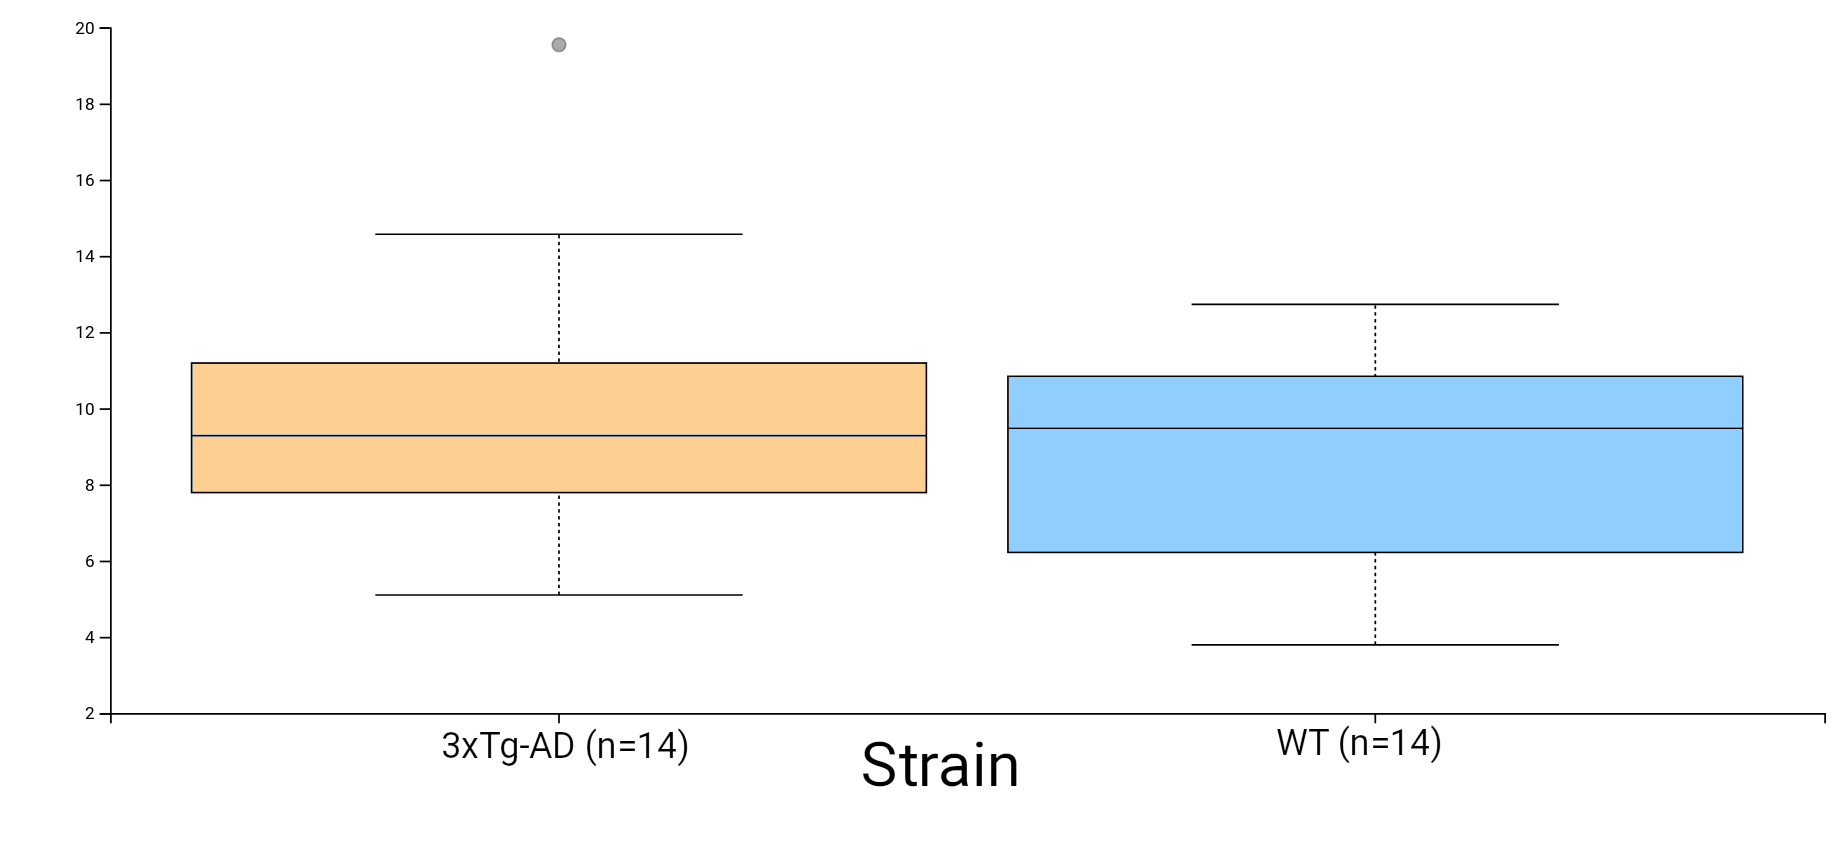
\includegraphics[width=.75\linewidth]{assets/faith_pd_group_sig_strain}}
    {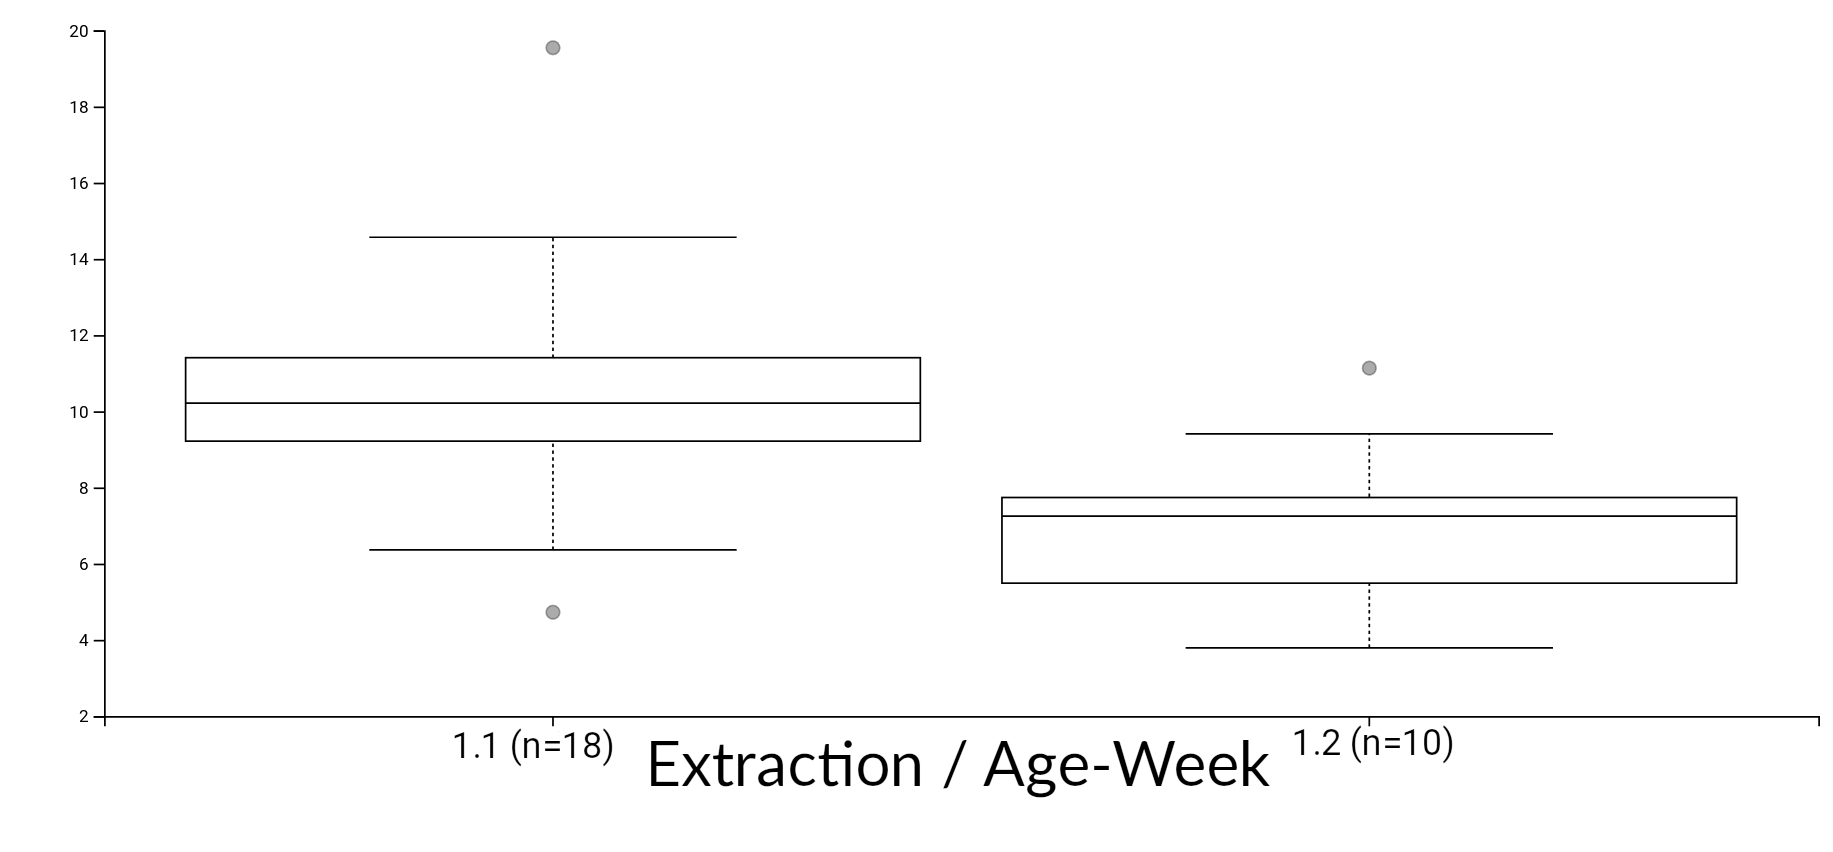
\includegraphics[width=.75\linewidth]{assets/faith_pd_group_sig_extraction}}
      \caption{\,When considering 8 and 24 week samples, alpha group
      significance plots of Faith's Phylogenetic Diversity show significant
      (p < 0.0035) differences across mouse age/extraction groups*, but no
      significant difference across strain}
      \label{fig:faith_strain}
    \end{figure}

  \end{block}

  \begin{block}{Discussion}
    Though complete longitudinal data are not yet available, the results
    to date support our hypothesis: qPCR data indicates that our most
    significant results are at 52 weeks, which is not unexected. We look
    forward to the sequencing of our final 16s data, and hope it supports the
    trends we see in qPCR.
  \end{block}

  \begin{block}{Future Work}

    \begin{itemize}
      \item \textbf{52-Week Analysis} Investigation of correlations between qPCR findings and 52-week 16s data
      \item \textbf{Immunohistochemistry} Quantification of neurofibrillary tangles and amyloid-β plaques
    \end{itemize}

  \end{block}

  % TODO: We'll deffo need references
  % Is it appropriate to qr-link our refs? The list from Q2 is likely to be long
  \begin{block}{References}
    References available at https://github.com/chriskeefe/urdea-poster/refs.bib
    % TODO: Replace this with an actual QR code
    
\includegraphics[height=5cm]{assets/repo}
    % \nocite{*}
    % \bibliographystyle{acm}\bibliography{poster}

  \end{block}

  \begin{figure}
    \begin{minipage}[c]{\textwidth}
      \hfill
      
\includegraphics[height=5cm]{assets/repo}
    \end{minipage}
    \begin{minipage}[c]{\textwidth}
      \hfill
      Poster Source: https://github.com/chriskeefe/urdea-poster
    \end{minipage}
\end{figure}


\end{column}

\separatorcolumn
\end{columns}
\end{frame}

\end{document}
